\documentclass[]{book}
\usepackage{lmodern}
\usepackage{amssymb,amsmath}
\usepackage{ifxetex,ifluatex}
\usepackage{fixltx2e} % provides \textsubscript
\ifnum 0\ifxetex 1\fi\ifluatex 1\fi=0 % if pdftex
  \usepackage[T1]{fontenc}
  \usepackage[utf8]{inputenc}
\else % if luatex or xelatex
  \ifxetex
    \usepackage{mathspec}
  \else
    \usepackage{fontspec}
  \fi
  \defaultfontfeatures{Ligatures=TeX,Scale=MatchLowercase}
\fi
% use upquote if available, for straight quotes in verbatim environments
\IfFileExists{upquote.sty}{\usepackage{upquote}}{}
% use microtype if available
\IfFileExists{microtype.sty}{%
\usepackage{microtype}
\UseMicrotypeSet[protrusion]{basicmath} % disable protrusion for tt fonts
}{}
\usepackage[margin=1in]{geometry}
\usepackage{hyperref}
\hypersetup{unicode=true,
            pdftitle={Jasonelle Documentation},
            pdfauthor={Jasonelle Team},
            pdfborder={0 0 0},
            breaklinks=true}
\urlstyle{same}  % don't use monospace font for urls
\usepackage{natbib}
\bibliographystyle{apalike}
\usepackage{longtable,booktabs}
\usepackage{graphicx,grffile}
\makeatletter
\def\maxwidth{\ifdim\Gin@nat@width>\linewidth\linewidth\else\Gin@nat@width\fi}
\def\maxheight{\ifdim\Gin@nat@height>\textheight\textheight\else\Gin@nat@height\fi}
\makeatother
% Scale images if necessary, so that they will not overflow the page
% margins by default, and it is still possible to overwrite the defaults
% using explicit options in \includegraphics[width, height, ...]{}
\setkeys{Gin}{width=\maxwidth,height=\maxheight,keepaspectratio}
\IfFileExists{parskip.sty}{%
\usepackage{parskip}
}{% else
\setlength{\parindent}{0pt}
\setlength{\parskip}{6pt plus 2pt minus 1pt}
}
\setlength{\emergencystretch}{3em}  % prevent overfull lines
\providecommand{\tightlist}{%
  \setlength{\itemsep}{0pt}\setlength{\parskip}{0pt}}
\setcounter{secnumdepth}{5}
% Redefines (sub)paragraphs to behave more like sections
\ifx\paragraph\undefined\else
\let\oldparagraph\paragraph
\renewcommand{\paragraph}[1]{\oldparagraph{#1}\mbox{}}
\fi
\ifx\subparagraph\undefined\else
\let\oldsubparagraph\subparagraph
\renewcommand{\subparagraph}[1]{\oldsubparagraph{#1}\mbox{}}
\fi

%%% Use protect on footnotes to avoid problems with footnotes in titles
\let\rmarkdownfootnote\footnote%
\def\footnote{\protect\rmarkdownfootnote}

%%% Change title format to be more compact
\usepackage{titling}

% Create subtitle command for use in maketitle
\newcommand{\subtitle}[1]{
  \posttitle{
    \begin{center}\large#1\end{center}
    }
}

\setlength{\droptitle}{-2em}

  \title{Jasonelle Documentation}
    \pretitle{\vspace{\droptitle}\centering\huge}
  \posttitle{\par}
    \author{Jasonelle Team}
    \preauthor{\centering\large\emph}
  \postauthor{\par}
      \predate{\centering\large\emph}
  \postdate{\par}
    \date{2018-11-25}

\usepackage{booktabs}

\begin{document}
\maketitle

{
\setcounter{tocdepth}{1}
\tableofcontents
}
\hypertarget{welcome}{%
\chapter{Welcome}\label{welcome}}

\emph{Jasonelle} Family is made of several components that share
\emph{JSON} as the main language.

\hypertarget{history}{%
\chapter{History}\label{history}}

\emph{Jasonette} was created by \emph{``Ethan Gliechtenstein''}, a New
York developer. Probably from Bushwick. Who's real identity nobody
knows.

\emph{Jasonette} core began in Late 2014 as an app named
\emph{``Ethan''} (\url{http://www.textethan.com/})

It got quickly popular.

\begin{itemize}
\item
  \url{https://twitter.com/Kelvin_T_/status/557001903851065346}
\item
  \url{https://techcrunch.com/2014/10/30/meet-samantha-ethan-apps-sister/}
\item
  \url{https://www.nytimes.com/2014/12/18/style/ethan-siri-meets-dr-phil.html}
\item
  \url{https://www.theguardian.com/technology/2014/dec/04/-sp-ten-best-messaging-apps}
\item
  \url{http://www.cnn.com/2014/10/11/tech/askethan-app}
\item
  \url{http://www.spiegel.de/netzwelt/apps/ask-ethan-app-beantwortet-fragen-der-nutzer-a-997335.html}
\item
  \url{http://www.newsnet5.com/the-now/some-guy-named-ethan-created-a-smartphone-app-ask-him-anything-and-get-answers}
\item
  \url{http://www.dazeddigital.com/artsandculture/article/22152/1/this-irl-siri-app-wants-to-answer-all-your-burning-questions}
\item
  \url{http://www.businessinsider.com/ethan-is-the-top-app-on-product-hunt-2014-10}
\item
  \url{http://www.sfgate.com/business/article/Stupid-apps-but-not-always-a-stupid-idea-5843629.php}
\end{itemize}

\begin{figure}
\centering
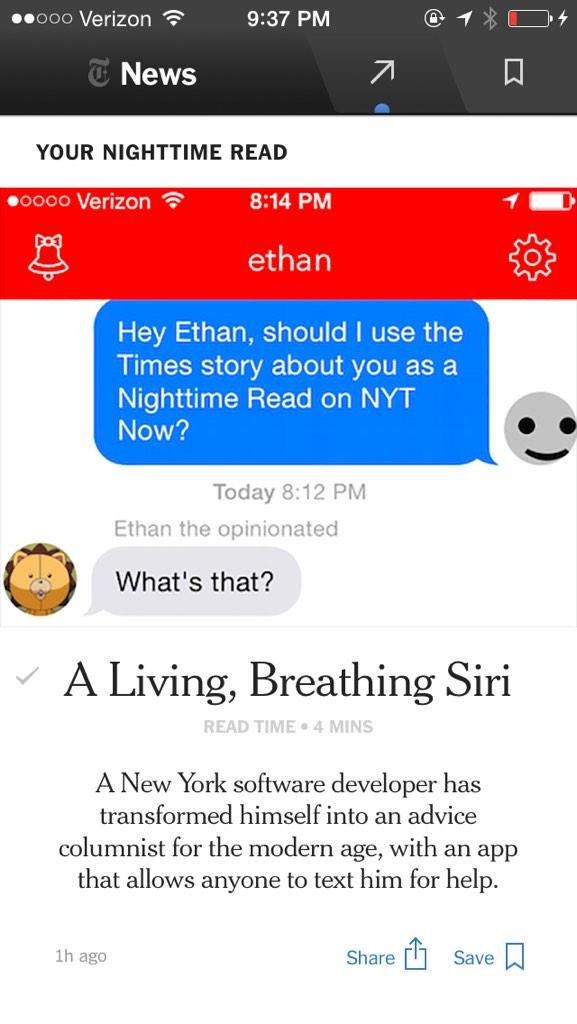
\includegraphics{images/history/ethanapp.jpeg}
\caption{Ethan App Screenshot}
\end{figure}

\begin{figure}
\centering

\includegraphics{images/history/ethan.jpeg}
\caption{Ethan Drawing}
\end{figure}

Some time after that Ethan began extracting the core, refining the api
and creating documentation.

After finally releasing the first version of Jasonette on November 3th
2016

\begin{itemize}
\item
  \url{https://www.producthunt.com/posts/jasonette}
\item
  \url{https://twitter.com/jasonclient/status/794175517763272708}
\end{itemize}

Ethan worked on \emph{Jasonette}, \emph{Cell} and \emph{ST} for nearly 2
years straight full-time. Until June 9 2018 were he misteriosly
disappeared without a trace. Later on November 6th 2018. \emph{Jasonelle
Team} took the lead.

The original repositories of \emph{Jasonette, Cell and ST} are:

\begin{itemize}
\tightlist
\item
  \url{https://github.com/jasonette}
\item
  \url{https://github.com/intercellular}
\item
  \url{https://github.com/selecttransform}
\end{itemize}

PD: If you want to know that character Ethan uses it's Kon from Bleach 💯
(\url{http://bleach.wikia.com/wiki/Kon})

\bibliography{book.bib,packages.bib}


\end{document}
